% Options for packages loaded elsewhere
\PassOptionsToPackage{unicode}{hyperref}
\PassOptionsToPackage{hyphens}{url}
%
\documentclass[
]{book}
\usepackage{amsmath,amssymb}
\usepackage{lmodern}
\usepackage{ifxetex,ifluatex}
\ifnum 0\ifxetex 1\fi\ifluatex 1\fi=0 % if pdftex
  \usepackage[T1]{fontenc}
  \usepackage[utf8]{inputenc}
  \usepackage{textcomp} % provide euro and other symbols
\else % if luatex or xetex
  \usepackage{unicode-math}
  \defaultfontfeatures{Scale=MatchLowercase}
  \defaultfontfeatures[\rmfamily]{Ligatures=TeX,Scale=1}
\fi
% Use upquote if available, for straight quotes in verbatim environments
\IfFileExists{upquote.sty}{\usepackage{upquote}}{}
\IfFileExists{microtype.sty}{% use microtype if available
  \usepackage[]{microtype}
  \UseMicrotypeSet[protrusion]{basicmath} % disable protrusion for tt fonts
}{}
\makeatletter
\@ifundefined{KOMAClassName}{% if non-KOMA class
  \IfFileExists{parskip.sty}{%
    \usepackage{parskip}
  }{% else
    \setlength{\parindent}{0pt}
    \setlength{\parskip}{6pt plus 2pt minus 1pt}}
}{% if KOMA class
  \KOMAoptions{parskip=half}}
\makeatother
\usepackage{xcolor}
\IfFileExists{xurl.sty}{\usepackage{xurl}}{} % add URL line breaks if available
\IfFileExists{bookmark.sty}{\usepackage{bookmark}}{\usepackage{hyperref}}
\hypersetup{
  pdftitle={Feasibility study on potential of data in financial services, Czech Republic},
  pdfauthor={Virginia Robano, under the supervision of Iota Nassr, OECD},
  hidelinks,
  pdfcreator={LaTeX via pandoc}}
\urlstyle{same} % disable monospaced font for URLs
\usepackage{longtable,booktabs,array}
\usepackage{calc} % for calculating minipage widths
% Correct order of tables after \paragraph or \subparagraph
\usepackage{etoolbox}
\makeatletter
\patchcmd\longtable{\par}{\if@noskipsec\mbox{}\fi\par}{}{}
\makeatother
% Allow footnotes in longtable head/foot
\IfFileExists{footnotehyper.sty}{\usepackage{footnotehyper}}{\usepackage{footnote}}
\makesavenoteenv{longtable}
\usepackage{graphicx}
\makeatletter
\def\maxwidth{\ifdim\Gin@nat@width>\linewidth\linewidth\else\Gin@nat@width\fi}
\def\maxheight{\ifdim\Gin@nat@height>\textheight\textheight\else\Gin@nat@height\fi}
\makeatother
% Scale images if necessary, so that they will not overflow the page
% margins by default, and it is still possible to overwrite the defaults
% using explicit options in \includegraphics[width, height, ...]{}
\setkeys{Gin}{width=\maxwidth,height=\maxheight,keepaspectratio}
% Set default figure placement to htbp
\makeatletter
\def\fps@figure{htbp}
\makeatother
\setlength{\emergencystretch}{3em} % prevent overfull lines
\providecommand{\tightlist}{%
  \setlength{\itemsep}{0pt}\setlength{\parskip}{0pt}}
\setcounter{secnumdepth}{5}
\usepackage{booktabs}
\usepackage{amsthm}
\makeatletter
\def\thm@space@setup{%
  \thm@preskip=8pt plus 2pt minus 4pt
  \thm@postskip=\thm@preskip
}
\makeatother
\ifluatex
  \usepackage{selnolig}  % disable illegal ligatures
\fi
\usepackage[]{natbib}
\bibliographystyle{apalike}

\title{Feasibility study on potential of data in financial services, Czech Republic}
\author{Virginia Robano, under the supervision of Iota Nassr, OECD}
\date{2022-05-01}

\begin{document}
\maketitle

{
\setcounter{tocdepth}{1}
\tableofcontents
}
\hypertarget{index}{%
\chapter*{Index}\label{index}}
\addcontentsline{toc}{chapter}{Index}

\hypertarget{purpose}{%
\chapter{Purpose}\label{purpose}}

\hypertarget{st-part-of-deliverables-by-30-june-2022}{%
\section*{1st part of deliverables by 30 June 2022:}\label{st-part-of-deliverables-by-30-june-2022}}
\addcontentsline{toc}{section}{1st part of deliverables by 30 June 2022:}

Identify good practices and business objectives for a regulatory framework supporting the development of FinTech

\begin{itemize}
\item
  Highlight key features of FinTech policy frameworks within other markets and any lessons learned, e.g.~with regards to data sharing projects, related standards and Open Banking initiatives already implemented elsewhere.
\item
  Create a set of Good Principles for Regulating New Technologies, including the process of defining new technologies, choosing the right regulatory approach and monitoring of the developments.
\item
  Define the set of key business objectives for the to-be Fintech environment to be achieved, in close cooperation with key stakeholders.
\end{itemize}

\hypertarget{nd-part-of-deliverables-by-31-october-2022}{%
\section*{2nd part of deliverables by 31 October 2022:}\label{nd-part-of-deliverables-by-31-october-2022}}
\addcontentsline{toc}{section}{2nd part of deliverables by 31 October 2022:}

Provide recommendations for effective supervision of the FinTech sector

\begin{itemize}
\item
  Analyse the past experience of competent authorities in financial services and supervisory solutions, mechanisms and practices existing in other similar countries in order to support efficient data sharing in financial services.
\item
  Propose/recommend SupTech methods and technologies to enable the flexible and effective supervision to address new supervisory challenges emerging from new risks, while avoiding to create an additional barrier, which could hinder the development of FinTech innovations.
\item
  Consider/Recommend creating additional dedicated programs on the central administration level (e.g innovation hubs, tax incentives or government programs enabling access to data).
\end{itemize}

\hypertarget{intro}{%
\chapter{Intro}\label{intro}}

\hypertarget{questions}{%
\section{Questions}\label{questions}}

\begin{itemize}
\item
  Why do we want this feasibility study?
\item
  Who are the stakeholders in favour?
\item
  What do we need to build a pilot project?
\item
  How can we ensure that the project is scalable?
\item
  What could be an alternative solution to a regulatory sandbox?
\item
  How big a slice of the pie can this pilot project solve?
\item
  How can we structure incentives adequately to entice behaviour?
\item
  How can we align incentives?
\item
  The illusion of knowledge
\end{itemize}

\hypertarget{context-and-objectives}{%
\chapter{Context and objectives}\label{context-and-objectives}}

\begin{itemize}
\item
  Administrative and regulatory reform
\item
  New business models
\end{itemize}

where every word counts; \texttt{new} as in \texttt{innovative\ products,\ processes\ or\ services}; \texttt{business} as in \texttt{a\ market-based\ solution}; and \texttt{models} as in \texttt{a\ sound\ theoretical\ foundation}.

\hypertarget{objectives}{%
\section{Objectives}\label{objectives}}

To assist authorities in increasing capacity to design, develop and implement reform.

\begin{quote}
The Czech Republic has requested support from the European Commission under Regulation (EU) 2021/240 establishing a Technical Support Instrument (``TSI Regulation'').
Following the assessment, the European Commission has decided to fund the request and provide technical support to the Czech Republic, together with the Organisation for Economic Co-operation and Development (OECD). The technical support will be provided in the area of administrative and regulatory reform, with the purpose of establishing a regulatory sandbox in the Czech Republic.
\end{quote}

\begin{quote}
According to the Financial Stability Board (FSB), Financial Technology (FinTech) can be defined as ``technology-enabled innovation in financial services that could result in new business models, applications, processes or products and could have an associated material effect on financial markets and institutions and how financial services are provided''. The key elements of this definition are: (i) a new technology, being the basis for the innovations, (ii) the disruptive nature of the innovations, (iii) the application of the innovations to the financial services.
\end{quote}

\begin{quote}
FinTech comprises a variety of products, applications, processes and business models that have transformed the traditional way of providing banking and financial services, which can be of great benefit to the Czech society (e.g (i) mobile/contactless payments and cross-border remittances, (ii) e-banking services, (iii) FinTech-assisted credit intermediation to SMEs and other financial services distributed by P2P or other FinTech platforms, (iv) crypto-assets and other distributed ledger technologies (DLT) -based financial applications, (v) artificial intelligence-based systems and machine learning models using big data for credit underwriting, algorithmic trading, asset management and other financial market applications).
\end{quote}

\begin{quote}
The Czech Republic lays the emphasis on the necessity (i) not to hinder the development of such promising and highly competitive new markets, (ii) while regulating them, so that consumer protection, market integrity, and financial stability are ensured.
\end{quote}

\hypertarget{relevance}{%
\section{Relevance}\label{relevance}}

This Action aims at supporting the growth of financial technologies by creating a regulatory sandbox with a dedicated testing data-sharing and data usage infrastructure. There is a need for a regulatory sandbox to test new products/services, while safeguarding all economic actors (investors, entrepreneurs, borrowers, lenders), from emerging risks and promote financial stability, the soundness of financial institutions and consumer protection.

A ``regulatory sandbox'' may be understood as a ``scheme to enable firms to test, pursuant to a specific testing plan agreed and monitored by a dedicated function of the competent authority, innovative financial products, financial services or business models.''

Activities to be performed:

• Output 1: Inception report.

• Output 2: Mapping report of the FinTech market in the Czech Republic.

• Output 3: Feasibility study report.

• Output 4: Recommendations report.

• Output 5: Final report

\hypertarget{responsibilities}{%
\subsection{Responsibilities:}\label{responsibilities}}

\begin{quote}
Following upon the methodology presented by the OECD during the kick-off meeting, the inception report should be produced covering all agreed operational aspects of the Action, in line with this Annex I. The report should cover, at least,
\end{quote}

\begin{itemize}
\item
  description of the detailed Action activities,
\item
  the timeline,
\item
  the information needs,
\item
  the communication arrangements,
\item
  possible external communication plans during the completion of the Action,
\item
  the feedback-processes for the Action,
\item
  potential risks associated with the implementation of the Action, as well as
\item
  the identification of responsible entities and actors that will need to provide the necessary information to the OECD.
\end{itemize}

\hypertarget{requests}{%
\section{Requests}\label{requests}}

\begin{quote}
Could you start thinking of methodological elements you would like to highlight for our presentation at the kick-off meeting, and send your suggestions by the end of this week?
\end{quote}

\begin{quote}
literature review
\end{quote}

\begin{quote}
\end{quote}

\hypertarget{scope-of-the-project}{%
\section{Scope of the project}\label{scope-of-the-project}}

\begin{quote}
administrative and regulatory reform, and consists of undertaking a feasibility study on the potential of data in financial services study and the establishment of a regulatory sandbox in the Czech Republic.
\end{quote}

Kick-off agenda

FinTech comprises a variety of products, applications, processes and business models that have transformed the traditional way of providing banking and financial services, which can be of great benefit to the Czech society (e.g.~mobile/contactless payments and cross-border remittances; e-banking services; FinTech-assisted credit intermediation to SMEs and other financial services distributed by P2P or other FinTech platforms; crypto-assets and other distributed ledger technologies (DLT) -based financial applications; artificial intelligence-based systems and machine learning models using big data for credit underwriting, algorithmic trading, asset management and other financial market applications).
FinTech can improve the efficiency of the financial sector, all the more so in the context of the digitalisation trend that was intensified during the Covid-19 pandemic. Modern technologies and the advantages of the Czech IT sector (technical capacities, skills) are not used to their full potential, and there is currently no innovation facilitator dedicated to financial technologies and data. The absence of legal certainty in the FinTech sector may hinder its full development, which could allow a greater use of digital services and thus enhance the growth potential of such markets.
Further promotion of FinTech innovation has the potential to provide important benefits to the Czech economy. Financial technologies can improve the efficiency of the financial system and deepen capital markets, drive productivity gains, promote competition in the financial services sector, and ultimately benefit small and medium-sized companies (SMEs) and financial consumers, while also advancing financial inclusion by allowing access to financial services for underserved and underbanked customers. The associated risks should be taken into careful consideration for each of the above, so that the potential of FinTech and data is unlocked while consumer protection, market integrity, and financial stability are ensured.
The project is highly linked to Chapter 1.4 of the Czech National Recovery and Resilience Plan which is focused on digital technologies and aims at creating sandboxes in regulated sectors in line with EU priorities.

\hypertarget{relevance-and-stakeholders}{%
\chapter{Relevance and stakeholders}\label{relevance-and-stakeholders}}

\begin{itemize}
\item
  Regulatory sandbox with dedicated testing-data sharing

  \begin{itemize}
  \tightlist
  \item
    data usage infrastructure
  \end{itemize}
\item
  Understand opportunities and risks of innovations, regulatory treatment
\item
  Assess viability

  \begin{itemize}
  \tightlist
  \item
    applications
  \item
    compliance
  \end{itemize}
\end{itemize}

\hypertarget{literature-review}{%
\section{Literature Review}\label{literature-review}}

Here is a review of existing methods.

\href{https://www.youtube.com/watch?v=tyN9CwJsQdg}{Susan Athey on the future of currency}

\href{https://tidy-finance.org/introduction-to-tidy-finance.html}{R book on tidy finance}
\#\# Singapore Financial Authority

\href{https://www.mas.gov.sg/development/fintech/regulatory-sandbox}{Singapore}

The FinTech Regulatory Sandbox framework enables financial institutions and FinTech players to experiment with innovative financial products or services in a live environment but within a well-defined space and duration.

Depending on the experiment, MAS will provide appropriate regulatory support by relaxing specific legal and regulatory requirements prescribed by MAS, which the sandbox entity will otherwise be subject to, for the duration of the sandbox.

The sandbox will include appropriate safeguards to contain the consequences of failure and maintain the overall safety and soundness of the financial system.

Upon successful experimentation and on exiting the sandbox, the sandbox entity must fully comply with the relevant legal and regulatory requirements.

\hypertarget{oecd-work-on-ai}{%
\section{OECD work on AI}\label{oecd-work-on-ai}}

\href{https://www.oecd.org/finance/artificial-intelligence-machine-learning-big-data-in-finance.htm}{AI in finance}

0/08/2021 - Artificial Intelligence (AI) techniques are being increasingly deployed in finance, in areas such as asset management, algorithmic trading, credit underwriting or blockchain-based finance, enabled by the abundance of available data and by affordable computing capacity. Machine learning (ML) models use big data to learn and improve predictability and performance automatically through experience and data, without being programmed to do so by humans.

The deployment of AI in finance is expected to increasingly drive competitive advantages for financial firms, by improving their efficiency through cost reduction and productivity enhancement, as well as by enhancing the quality of services and products offered to consumers. These competitive advantages can, in turn, benefit financial consumers by providing increased quality and personalised products, unlocking insights from data to inform investment strategies and potentially enhancing financial inclusion by allowing for the analysis of creditworthiness of clients with limited credit history (e.g.~thin file SMEs).

At the same time, AI applications in finance may create or intensify financial and non-financial risks, and give rise to potential financial consumer and investor protection considerations (e.g.~as risks of biased, unfair or discriminatory consumer results, or data management and usage concerns). The lack of explainability of AI model processes could give rise to potential pro-cyclicality and systemic risk in the markets, and could create possible incompatibilities with existing financial supervision and internal governance frameworks, possibly challenging the technology-neutral approach to policymaking. While many of the potential risks associated with AI in finance are not unique to this innovation, the use of such techniques could amplify these vulnerabilities given the extent of complexity of the techniques employed, their dynamic adaptability and their level of autonomy.

The report can help policy makers to assess the implications of these new technologies and to identify the benefits and risks related to their use. It suggests policy responses that that are intended to support AI innovation in finance while ensuring that its use is consistent with promoting financial stability, market integrity and competition, while protecting financial consumers. Emerging risks from the deployment of AI techniques need to be identified and mitigated to support and promote the use of responsible AI. Existing regulatory and supervisory requirements may need to be clarified and sometimes adjusted, as appropriate, to address some of the perceived incompatibilities of existing arrangements with AI applications.

\hypertarget{non-fungible-tokens}{%
\section{Non Fungible Tokens}\label{non-fungible-tokens}}

NFTs create digital scarcity. This occurs as soon as it is possible to identify the property of something. It can be a work of art, an image, a document, a collectible, a portfolio image, a newspaper article or a Twitter post. By digitally identifying property, they become verifiable, programmable, divisible, durable, combinable, and easily transferable items.

NFTs opens up a wide range of new forms of business and new customs. It impacts all content creation industries, such as art, music, or publishing. In addition, it opens up possibilities for registering physical things, such as validations of study titles.

It is not only about being the owner of an image, but also about the identity of each one, about being able to access communities, the Metaverse and new ways of social organisation.
NFTs will even have impacts on the future of work.

\hypertarget{literature-review-on-google-scholar}{%
\section{Literature review on google scholar}\label{literature-review-on-google-scholar}}

\hypertarget{against-sandboxes-and-pro-innovation-hubs}{%
\subsection{Against sandboxes and pro innovation hubs}\label{against-sandboxes-and-pro-innovation-hubs}}

\begin{itemize}
\tightlist
\item
  negative outlook
\end{itemize}

\citet{buckley2020building}
Around the world, regulators and policymakers are working to support the development of financial technology (FinTech) ecosystems. As one example, more than fifty jurisdictions have now established or announced ``financial regulatory sandboxes.'' Others have announced or established ``innovation hubs,'' sometimes incorporating a regulatory sandbox as one element. This article argues that innovation hubs provide all the benefits that the policy discussion associates with regulatory sandboxes, while avoiding most downsides of regulatory sandboxes, and that many benefits typically attributed to sandboxes are the result of inconsistent terminology, and actually accrue from the work of innovation hubs. The paper presents, as the first contribution of its kind, data on regulatory sandboxes and innovation hubs and argues that the data so far available on sandboxes does not justify the statement that regulatory sandboxes are the most effective approach to building FinTech ecosystems. Given that regulatory sandboxes require significant financial contributions, sometimes new legislation, and intense regulatory risk management, and that they do not work as well on a stand-alone basis (i.e.~without an innovation hub), while innovation hubs alone can provide more significant benefits in support the development of a FinTech ecosystem, regulators should focus their resources on developing effective innovation hubs, including, in appropriate cases, a sandbox as one possible element.

\url{https://journals.library.wustl.edu/lawpolicy/article/id/750/}

\begin{itemize}
\tightlist
\item
  negative outlook
\end{itemize}

\citet{brown2022governing}
This article evaluates the sandbox approach as a regulatory answer to the challenges financial technology brings to finance and social relations. Taking fintech as a sociotechnological phenomenon embedded in discourses of solutionism and innovation, we show that the regulatory sandbox accepts these discourses. Instead of containing fintech, the sandbox is designed in a way that advances riskwashing of fintech even if it is disguised as risktaming. Next, we demonstrate fintech's problematic nature that regulation should control.

First, we propose that \textbf{through its information processing capacity, fintech accelerates the transition from bank-based to market-based finance.}

Second, we demonstrate that \textbf{fintech as part of a fintech-financialization apparatus has catallactic and value-extracting governance effects.}

Third, inserting the fintech-financialization apparatus into Fourcade and Healy's argument on the social stratification effect of the data-driven economy, \textbf{we argue that it also has a socially disruptive potential.} We critique the regulatory sandbox for being a facilitator to this process and recommend increasing the number and power of veto players and veto points in complex regulatory regimes.

\begin{itemize}
\tightlist
\item
  positive outlook
\end{itemize}

\citet{bromberg2017fintech}
The growth of Fintech, which refers to the use of technology in providing financial services, is continuing to disrupt global financial services markets. The rapidly evolving technological landscape provides challenges for financial regulators, which are already facing the need to address a broader set of regulatory objectives and policy priorities following the Global Financial Crisis (GFC). Regulatory sandboxes, which are aimed at encouraging innovation by allowing businesses to test their Fintech offerings in a `safe' environment, provide an example of a shift away from traditional regulatory approaches and represent an attempt to embrace principles of proactive, dynamic and responsive regulation. This article examines key differences between the sandbox regimes that have been implemented to date, and explores the implications of sandboxes for businesses, consumers and domestic regulators.

\begin{center}\rule{0.5\linewidth}{0.5pt}\end{center}

\hypertarget{natural-language-processing}{%
\section{Natural Language Processing}\label{natural-language-processing}}

\hypertarget{pdf-documents}{%
\subsection{6 PDF Documents}\label{pdf-documents}}

Michaela's favourite EU materials on regulatory sandboxes (very important for the understanding the EU licensing framework):

Regulatory Sandboxes: a Technical Guide CGAP
\href{https://www.cgap.org/research/publication/how-build-regulatory-sandbox-practical-guide-policy-makers}{PDF1}

PDF2: Annex I: Description of the Action Plan OECD (PDF sent by Iota)

\href{https://www.esma.europa.eu/sites/default/files/library/esma50-164-2430_licensing_of_fintech.pdf}{PDF3}

\href{https://www.europarl.europa.eu/RegData/etudes/STUD/2020/652752/IPOL_STU(2020)652752_EN.pdf}{PDF4}

\href{https://esas-joint-committee.europa.eu/Publications/Reports/JC\%202018\%2074\%20Joint\%20Report\%20on\%20Regulatory\%20Sandboxes\%20and\%20Innovation\%20Hubs.pdf}{PDF5}

\href{https://data.consilium.europa.eu/doc/document/ST-13026-2020-INIT/en/pdf}{PDF6}
Proceedings of the European Commission

\hypertarget{analysis}{%
\subsection{Analysis}\label{analysis}}

\begin{figure}

{\centering 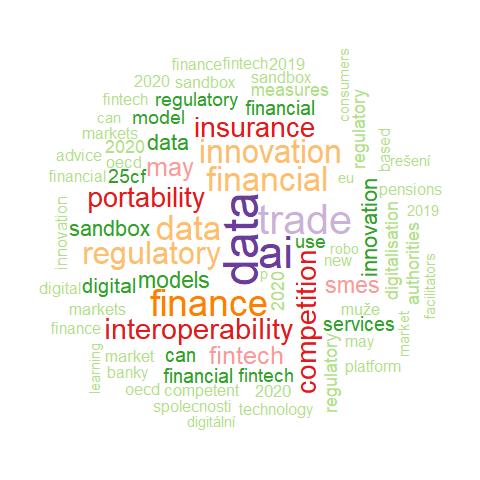
\includegraphics[width=0.8\linewidth]{img/nube} 

}

\caption{Wordcloud}\label{fig:nice-figN1}
\end{figure}

\begin{figure}

{\centering 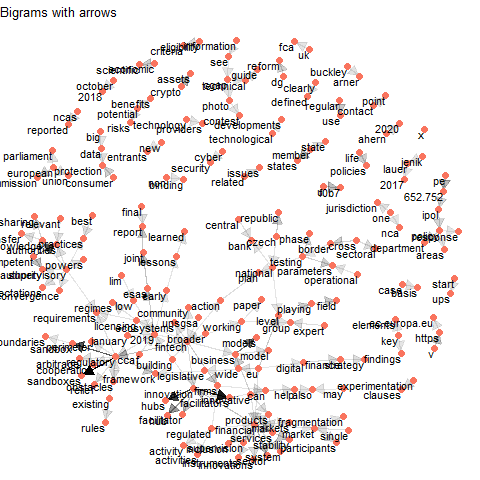
\includegraphics[width=0.8\linewidth]{img/bigrams3} 

}

\caption{Bigrams in all 6 PDF texts}\label{fig:nice-figB1}
\end{figure}

Regulatory Sandboxes: a Technical Guide CGAP
\href{https://www.cgap.org/research/publication/how-build-regulatory-sandbox-practical-guide-policy-makers}{PDF1}

\begin{figure}

{\centering 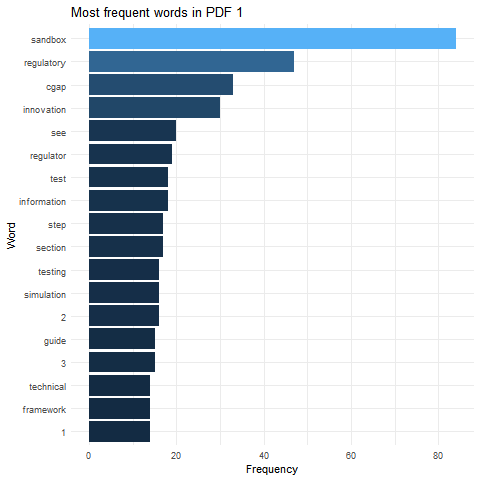
\includegraphics[width=0.8\linewidth]{img/freqP1} 

}

\caption{Bigrams in all 6 PDF texts}\label{fig:nice-figF1}
\end{figure}

PDF2: Annex I: Description of the Action Plan OECD (PDF sent by Iota)

\begin{figure}

{\centering 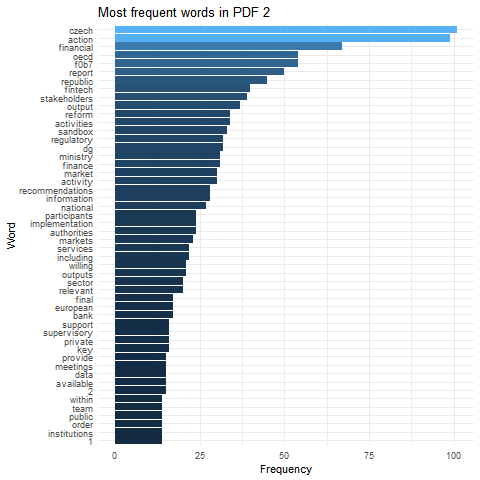
\includegraphics[width=0.8\linewidth]{img/freqP2} 

}

\caption{Bigrams in all 6 PDF texts}\label{fig:nice-figF2}
\end{figure}

\href{https://www.esma.europa.eu/sites/default/files/library/esma50-164-2430_licensing_of_fintech.pdf}{PDF3}

\begin{figure}

{\centering 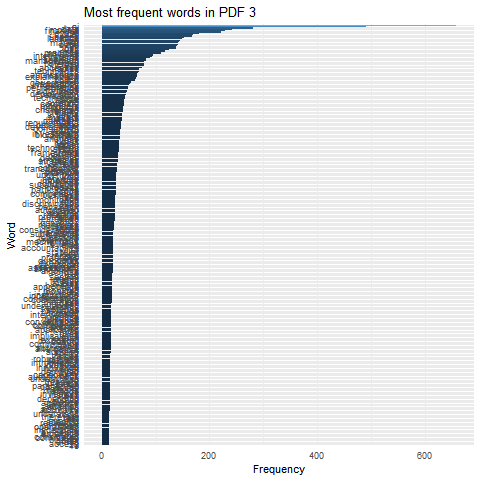
\includegraphics[width=0.8\linewidth]{img/freqP3} 

}

\caption{Bigrams in all 6 PDF texts}\label{fig:nice-figF3}
\end{figure}

\href{https://www.europarl.europa.eu/RegData/etudes/STUD/2020/652752/IPOL_STU(2020)652752_EN.pdf}{PDF4}

\begin{figure}

{\centering 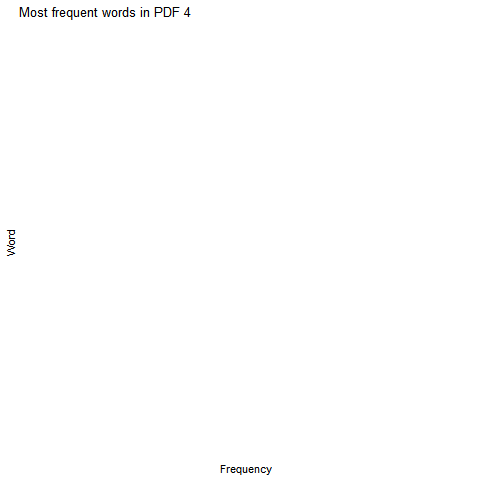
\includegraphics[width=0.8\linewidth]{img/freqP4} 

}

\caption{Bigrams in all 6 PDF texts}\label{fig:nice-figF4}
\end{figure}

\href{https://esas-joint-committee.europa.eu/Publications/Reports/JC\%202018\%2074\%20Joint\%20Report\%20on\%20Regulatory\%20Sandboxes\%20and\%20Innovation\%20Hubs.pdf}{PDF5}

\begin{figure}

{\centering 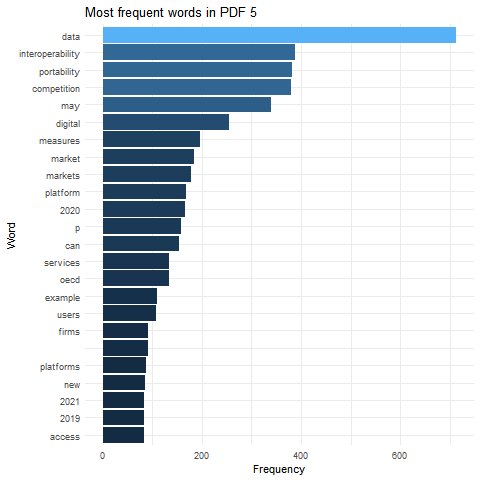
\includegraphics[width=0.8\linewidth]{img/freqP5} 

}

\caption{Bigrams in all 6 PDF texts}\label{fig:nice-figF5}
\end{figure}

\href{https://data.consilium.europa.eu/doc/document/ST-13026-2020-INIT/en/pdf}{PDF6}
Proceedings of the European Commission

\begin{figure}

{\centering 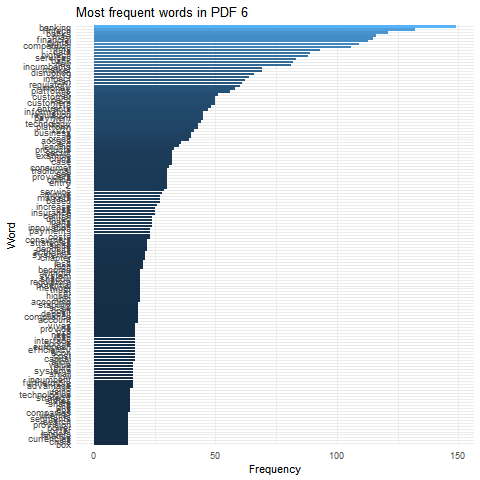
\includegraphics[width=0.8\linewidth]{img/freqP6} 

}

\caption{Bigrams in all 6 PDF texts}\label{fig:nice-figF6}
\end{figure}

\hypertarget{new-documents}{%
\section{New documents}\label{new-documents}}

\href{https://data.consilium.europa.eu/doc/document/ST-13026-2020-INIT/en/pdf}{PDF7}
Proceedings of the European Commission

\begin{figure}

{\centering 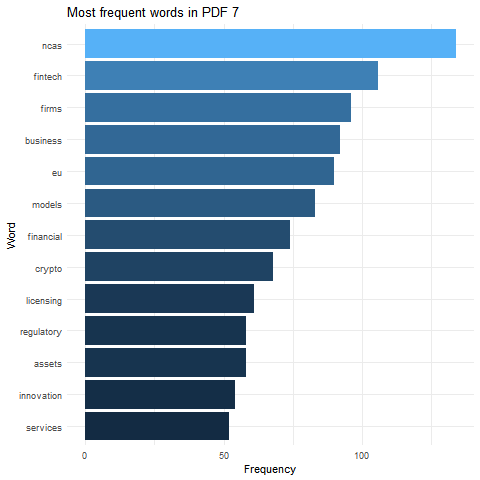
\includegraphics[width=0.8\linewidth]{img/freqP7} 

}

\caption{Bigrams in all 6 PDF texts}\label{fig:nice-figF7-16-1}
\end{figure}
\begin{figure}

{\centering 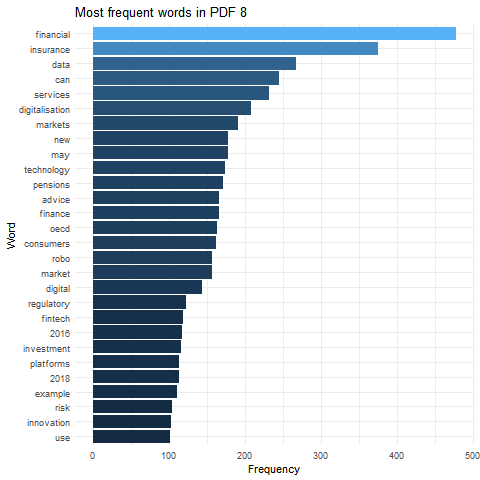
\includegraphics[width=0.8\linewidth]{img/freqP8} 

}

\caption{Bigrams in all 6 PDF texts}\label{fig:nice-figF7-16-2}
\end{figure}
\begin{figure}

{\centering 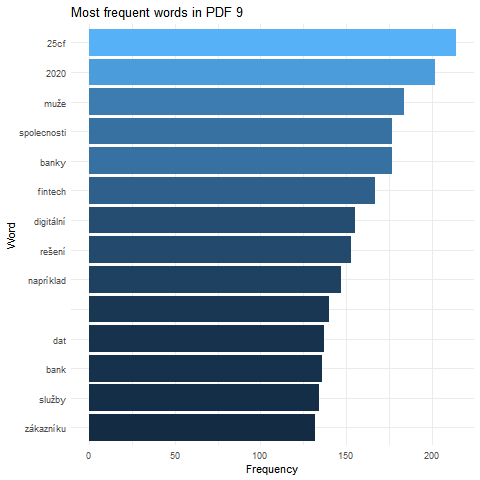
\includegraphics[width=0.8\linewidth]{img/freqP9} 

}

\caption{Bigrams in all 6 PDF texts}\label{fig:nice-figF7-16-3}
\end{figure}
\begin{figure}

{\centering 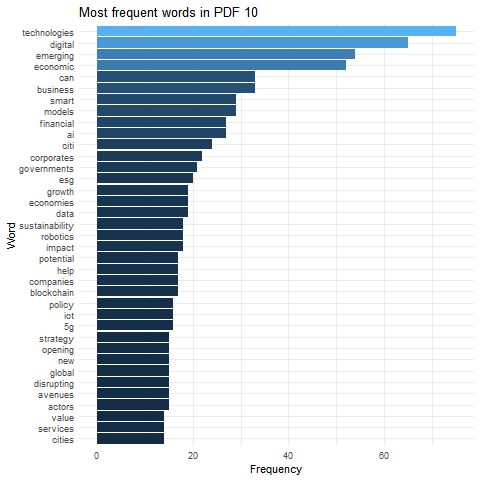
\includegraphics[width=0.8\linewidth]{img/freqP10} 

}

\caption{Bigrams in all 6 PDF texts}\label{fig:nice-figF7-16-4}
\end{figure}
\begin{figure}

{\centering 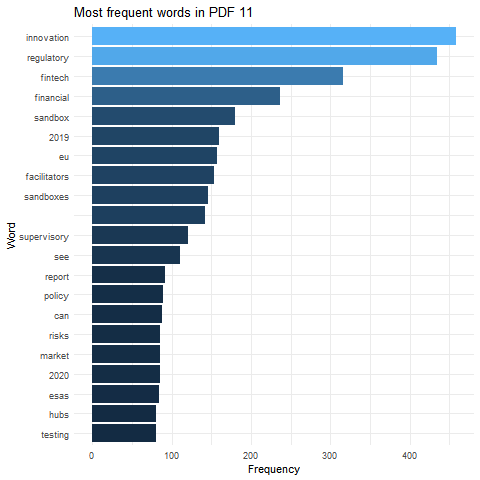
\includegraphics[width=0.8\linewidth]{img/freqP11} 

}

\caption{Bigrams in all 6 PDF texts}\label{fig:nice-figF7-16-5}
\end{figure}
\begin{figure}

{\centering 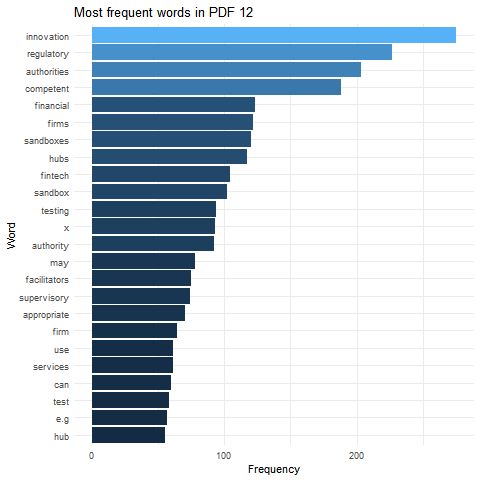
\includegraphics[width=0.8\linewidth]{img/freqP12} 

}

\caption{Bigrams in all 6 PDF texts}\label{fig:nice-figF7-16-6}
\end{figure}
\begin{figure}

{\centering 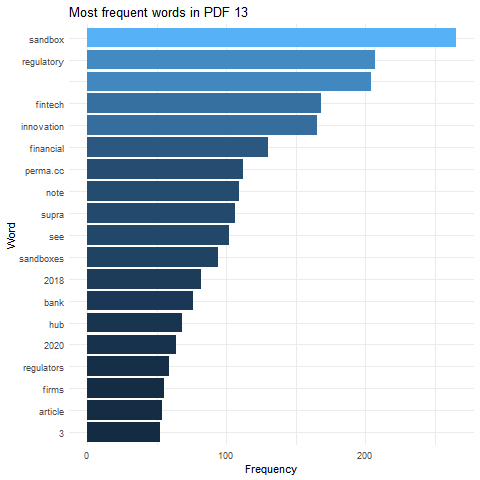
\includegraphics[width=0.8\linewidth]{img/freqP13} 

}

\caption{Bigrams in all 6 PDF texts}\label{fig:nice-figF7-16-7}
\end{figure}
\begin{figure}

{\centering 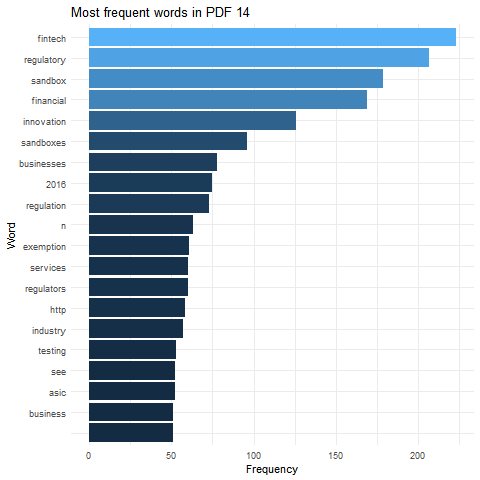
\includegraphics[width=0.8\linewidth]{img/freqP14} 

}

\caption{Bigrams in all 6 PDF texts}\label{fig:nice-figF7-16-8}
\end{figure}
\begin{figure}

{\centering 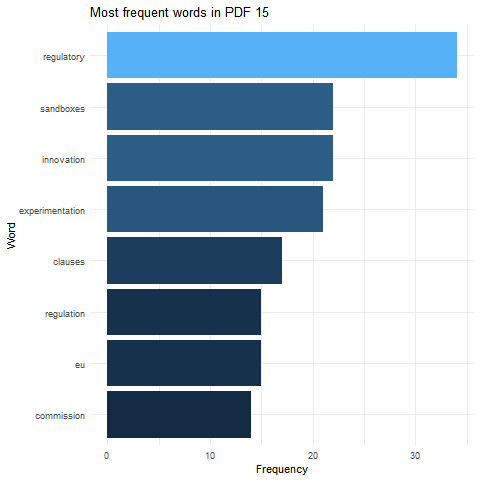
\includegraphics[width=0.8\linewidth]{img/freqP15} 

}

\caption{Bigrams in all 6 PDF texts}\label{fig:nice-figF7-16-9}
\end{figure}
\begin{figure}

{\centering 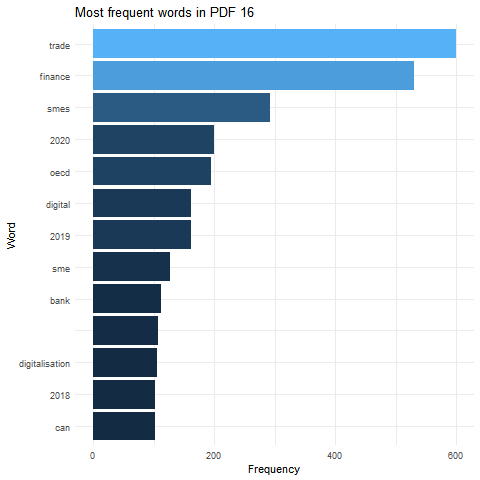
\includegraphics[width=0.8\linewidth]{img/freqP16} 

}

\caption{Bigrams in all 6 PDF texts}\label{fig:nice-figF7-16-10}
\end{figure}

\begin{figure}

{\centering 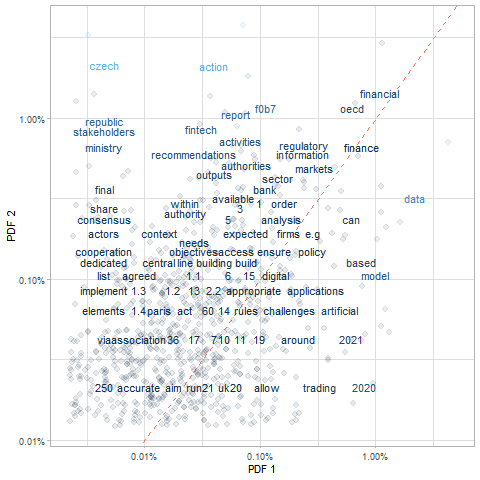
\includegraphics[width=0.8\linewidth]{img/p1p2} 

}

\caption{Wordcloud}\label{fig:nice-figjapN2-1}
\end{figure}
\begin{figure}

{\centering 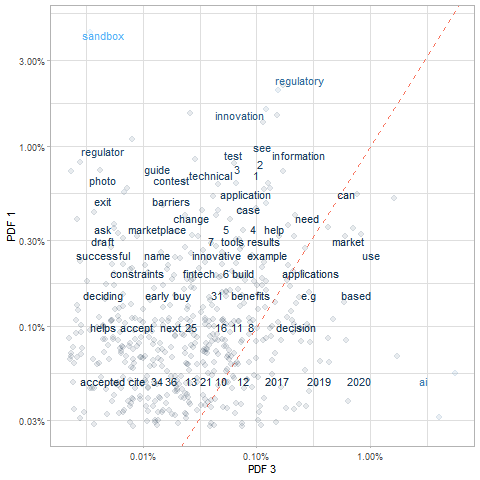
\includegraphics[width=0.8\linewidth]{img/p1p3} 

}

\caption{Wordcloud}\label{fig:nice-figjapN2-2}
\end{figure}
\begin{figure}

{\centering 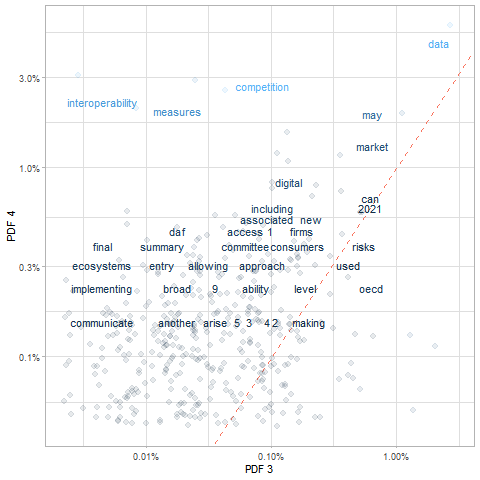
\includegraphics[width=0.8\linewidth]{img/p1p4} 

}

\caption{Wordcloud}\label{fig:nice-figjapN2-3}
\end{figure}
\begin{figure}

{\centering 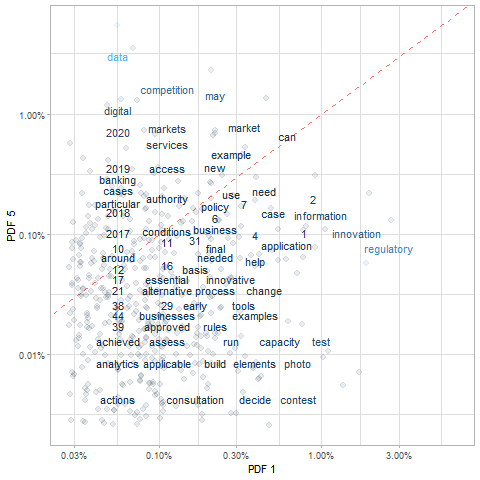
\includegraphics[width=0.8\linewidth]{img/p1p5} 

}

\caption{Wordcloud}\label{fig:nice-figjapN2-4}
\end{figure}
\begin{figure}

{\centering 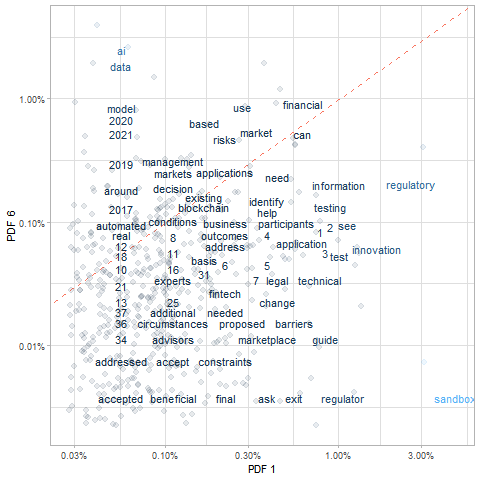
\includegraphics[width=0.8\linewidth]{img/p1p6} 

}

\caption{Wordcloud}\label{fig:nice-figjapN2-5}
\end{figure}
\begin{figure}

{\centering 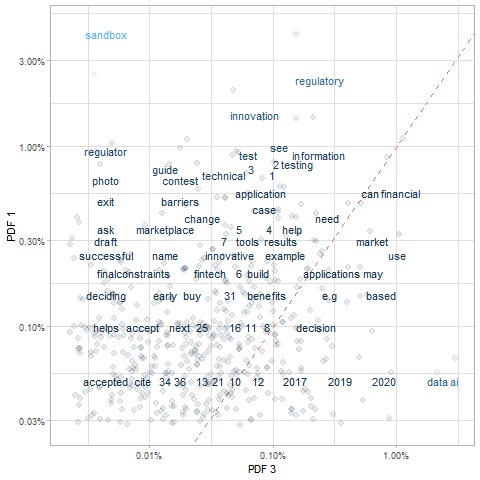
\includegraphics[width=0.8\linewidth]{img/p3p1} 

}

\caption{Wordcloud}\label{fig:nice-figjapN2-6}
\end{figure}
\begin{figure}

{\centering 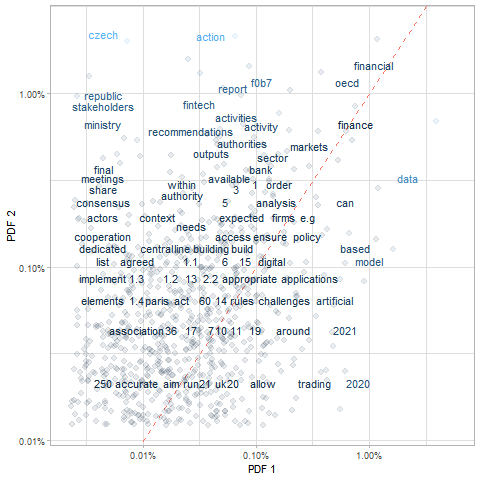
\includegraphics[width=0.8\linewidth]{img/p3p2} 

}

\caption{Wordcloud}\label{fig:nice-figjapN2-7}
\end{figure}
\begin{figure}

{\centering 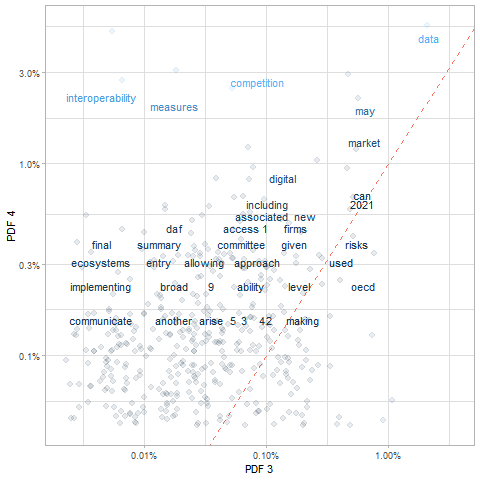
\includegraphics[width=0.8\linewidth]{img/p3p4} 

}

\caption{Wordcloud}\label{fig:nice-figjapN2-8}
\end{figure}

\begin{figure}

{\centering 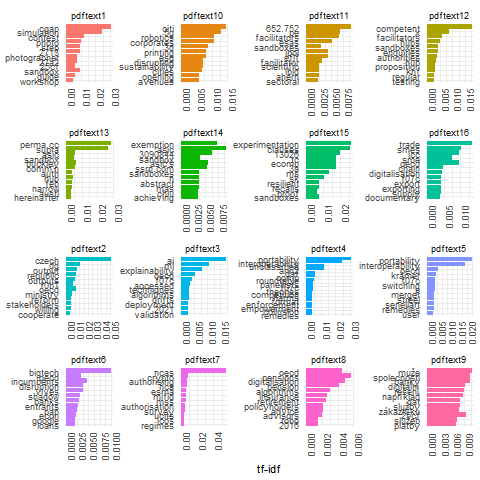
\includegraphics[width=0.8\linewidth]{img/tf_idf} 

}

\caption{Comparison of frequencies}\label{fig:nice-figN3}
\end{figure}

Financial technology, or fintech, is developing at a rapid rate, disrupting sectors as diverse as corporates, banking, trading and investment, personal finance, accounting, and insurance. More broadly, it challenges our notions of money and value and our understanding of the impact of technology on finance, business, and society.

By virtue of technical advances such as cloud computing, mobile communication, machine learning, blockchains and data science, fintech is transforming the business of finance: it allows the reimagining of current systems, the creation of novel products and services, and automation to better serve businesses and society. Greater global interconnectivity means fintech is making financial services accessible to a larger global population than ever, presenting both game-changing societal opportunities and novel risks.

\href{https://www.imperial.ac.uk/business-school/faculty-research/research-centres/centre-financial-technology/}{Imperial College: Centre for Financial technology}

\hypertarget{netherlands}{%
\subsection{\texorpdfstring{\href{https://www.afm.nl/en/professionals/onderwerpen/innovationhub-maatwerk}{Netherlands}}{Netherlands}}\label{netherlands}}

\hypertarget{methodology}{%
\chapter{Methodology}\label{methodology}}

\hypertarget{desk-research}{%
\section{Desk research}\label{desk-research}}

\hypertarget{academic-literature-review}{%
\section{Academic literature review}\label{academic-literature-review}}

\hypertarget{peer-review-of-existing-sandboxes}{%
\section{Peer review of existing sandboxes}\label{peer-review-of-existing-sandboxes}}

\begin{itemize}
\item
  Netherlands
\item
  United Kingdom
\item
  Singapore
\end{itemize}

\hypertarget{action-impact-and-outcome}{%
\chapter{Action impact and outcome}\label{action-impact-and-outcome}}

\hypertarget{contribution-towards-the-creation-of-an-incentive-ecosystem-for-fintechs-start-ups-and-incumbent-firms}{%
\section{Contribution towards the creation of an incentive ecosystem for FinTechs, start-ups and incumbent firms}\label{contribution-towards-the-creation-of-an-incentive-ecosystem-for-fintechs-start-ups-and-incumbent-firms}}

\hypertarget{output-and-activities}{%
\section{Output and activities}\label{output-and-activities}}

\begin{enumerate}
\def\labelenumi{\arabic{enumi}.}
\item
  Inception report
\item
  Mapping
\item
  Feasibility
\item
  Recommendations
\item
  Final
\end{enumerate}

\begin{center}\rule{0.5\linewidth}{0.5pt}\end{center}

\hypertarget{issues}{%
\section{Issues}\label{issues}}

\hypertarget{data-quality-and-data-management}{%
\subsection{Data quality and data management}\label{data-quality-and-data-management}}

\begin{quote}
Data is a key component of all these innovative FinTech mechanisms:
alternative data and big data are being used by FinTech intermediaries to allow
for the extension of financing to thin file customers and SMEs without
collateral; customer-permissioned financial data are being shared by
intermediaries with other parties and firms to build innovative applications and
services in payments and other domains; while artificial intelligence and
machine learning models can only be useful if fed with massive amounts of
good quality, adequate data.
\end{quote}

\begin{quote}
Sandboxes across Europe and the world have proved to constitute an excellent
way for financial authorities to accompany the development of innovative
financial solutions in a safe and controlled manner. And let me stress that
carefully designed sandboxes are regulated environments that should not be
perceived as a testing ground where laws and regulations do not apply. Rather,
their purpose is to enable market participants and supervisors to engage in a
constructive dialogue that helps strike the right balance between financial
innovation and mitigation of ensuing risks.
\end{quote}

\hypertarget{co-participation-co--creation}{%
\subsection{Co participation \textbar{} Co- creation}\label{co-participation-co--creation}}

\hypertarget{what-are-the-reasons-this-will-not-work}{%
\subsection{What are the reasons this will not work?}\label{what-are-the-reasons-this-will-not-work}}

How can we lift them?

\hypertarget{final-words}{%
\chapter{Final Words}\label{final-words}}

We have finished a nice report.

\hypertarget{stakeholders}{%
\chapter{Stakeholders}\label{stakeholders}}

\hypertarget{czechia}{%
\section{Czechia}\label{czechia}}

• Mr Jiří Georgiev, Deputy Minister of Finance of the Czech Republic

• Deputy Governor of the Czech National Bank {[}TBD{]}

\begin{itemize}
\item
  Ivančo Alex JUDr. Ph.D.~\href{mailto:Alex.Ivanco@mfcr.cz}{\nolinkurl{Alex.Ivanco@mfcr.cz}};
  Alex Ivanco|\href{mailto:Alex.Ivanco@mfcr.cz}{\nolinkurl{Alex.Ivanco@mfcr.cz}}
  Director, Ministry of Finance of the Czech Republic
\item
  Franče Rejzková Lenka JUDr. \href{mailto:Lenka.France_Rejzkova@mfcr.cz}{\nolinkurl{Lenka.France\_Rejzkova@mfcr.cz}};
  Lenka Franče Rejzková|\href{mailto:Lenka.France_Rejzkova@mfcr.cz}{\nolinkurl{Lenka.France\_Rejzkova@mfcr.cz}}
  Ministry of Finance of the Czech Republic
\item
  Soukupová Marie \href{mailto:Marie.Soukupova@mfcr.cz}{\nolinkurl{Marie.Soukupova@mfcr.cz}};
\end{itemize}

\hypertarget{european-commission}{%
\section{European Commission}\label{european-commission}}

\href{https://www.linkedin.com/in/\%C3\%A9douard-gomet-a4a19761/?originalSubdomain=fr}{Édouard Gomet}
- GOMET Edouard (REFORM) \href{mailto:Edouard.GOMET@ec.europa.eu}{\nolinkurl{Edouard.GOMET@ec.europa.eu}}
Edouard Gomet |Edouard.Gomet@ ec.europa.eu
European Commission, Directorate-General for Structural Reform Support
REFORM Unit B5 -- Financial sector and access to finance

\begin{itemize}
\item
  RINALDI Laura (REFORM) \href{mailto:Laura.RINALDI@ec.europa.eu}{\nolinkurl{Laura.RINALDI@ec.europa.eu}};
\item
  TSCHIRKOVA Gabriela (REFORM) \href{mailto:Gabriela.TSCHIRKOVA@ec.europa.eu}{\nolinkurl{Gabriela.TSCHIRKOVA@ec.europa.eu}};
\end{itemize}

• Mr Mario Nava, Director-General DG Reform (virtual)

\hypertarget{oecd}{%
\section{OECD}\label{oecd}}

• Mr Carmine Di Noia, Director, OECD Directorate for Financial and Enterprise Affairs (virtual)

\begin{itemize}
\tightlist
\item
  Rob Palatano Acting head of DAF FM
  Robert Patalano |\href{mailto:Robert.Patalano@oecd.org}{\nolinkurl{Robert.Patalano@oecd.org}}
  Directorate for Financial and Enterprise Affairs, OECD
  Head of the Financial Markets Division
\end{itemize}

Iota Nassr |\href{mailto:Iota.Nassr@oecd.org}{\nolinkurl{Iota.Nassr@oecd.org}}
Directorate for Financial and Enterprise Affairs, OECD
Financial Markets Division

• Ms Iota Nassr, OECD

• Ms Ana Sasi-Brodesky, OECD

• Ms Virginia Robano, OECD

• Ms Michala Stupkova, OECD
- Stupková Michala \href{mailto:Michala.Stupkova@mfcr.cz}{\nolinkurl{Michala.Stupkova@mfcr.cz}}; Michala Stupková \href{mailto:michala.stupkova@gmail.com}{\nolinkurl{michala.stupkova@gmail.com}}

  \bibliography{book.bib}

\end{document}
